\section{Resultados}\label{sec:resultados}

Os resultados mais relevantes obtidos estão apresentados nesta seção e estruturados de maneira que, para cada uma das configurações mencionadas, e algumas das métricas descritas na Seção~\ref{sec:metodologia-metricas}, são apresentadas as curvas de médias cumulativas e estimativas de densidade por núcleo (KDE), além dos respectivos resultados dos testes de significância estatística. 

\subsection{Resultados Considerando Todas as Camadas de Ativações}\label{sec:resultados-complete}

A seguir, estão apresentados os resultados da configuração que considerou as ativações de todas as camadas, capturadas com a biblioteca LLM-MRI, gerados a partir da entrada dos prompts de labirintos pelos modelos.

\begin{itemize}
    \item \textbf{Número de Nós ($|V|$) e Número de Arestas ($|E|$)}: não foram observadas diferenças significativas entre os modelos, resultando em distribuições bastante similares e com pouca variabilidade entre os experimentos realizados. Dessa forma, não foram incluídas figuras para estas métricas.
\end{itemize}

\subsubsection{Grau Médio ($\bar{k}$)}

A média cumulativa dos graus médios obtidos para os três modelos, considerando todas as camadas, estão apresentados na Figura~\ref{fig:complete-cumulative-mean-grau-medio}. Na qual, observa-se que as curvas convergem para valores próximos, indicando, ao final, uma média estável maior para o modelo ajustado com GRPO, seguido do modelo Base e, por fim, o modelo ajustado com SFT.

\begin{figure}[h!]
    \centering
    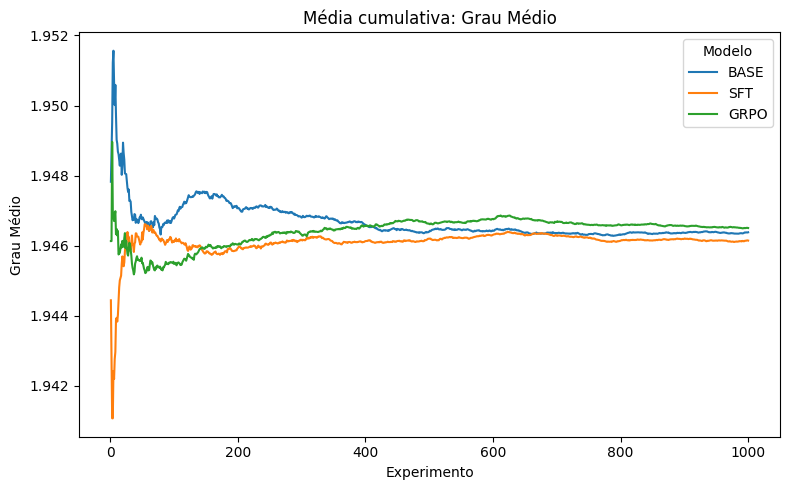
\includegraphics[width=0.75\textwidth]{figure/complete/cumulative-mean/grau-medio.png}
    \caption{Média cumulativa do Grau Médio ($\bar{k}$).}
    \label{fig:complete-cumulative-mean-grau-medio}
\end{figure}


Na Figura~\ref{fig:complete-kde-grau-medio}, observa-se que os três modelos apresentaram distribuições bastante similares para o KDE do grau médio. Apesar de médias muito próximas, pode-se notar que o modelo os modelos ajustados, SFT e GRPO, exibem um pico ligeiramente mais acentuado em relação ao modelo Base, sugerindo uma maior concentração de valores em torno da média, com este último apresentando uma distribuição levemente mais à esquerda.

\begin{figure}[h!]
    \centering
    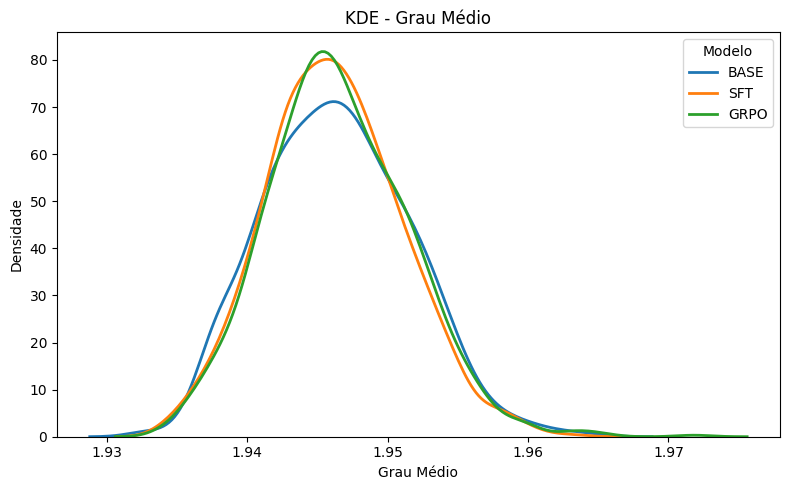
\includegraphics[width=0.75\textwidth]{figure/complete/kde/grau-medio.png}
    \caption{KDE do Grau Médio ($\bar{k}$).}
    \label{fig:complete-kde-grau-medio}
\end{figure}

\subsubsection{Densidade ($\rho$)}

Nota-se, ao analisar a figura da média cumulativa da densidade do grafo das ativações na Figura~\ref{fig:complete-cumulative-mean-densidade} que, novamente, os três modelos convergem para valores muito próximos com GRPO apresentando a maior média, seguido do modelo Base e SFT.

\begin{figure}[h!]
    \centering
    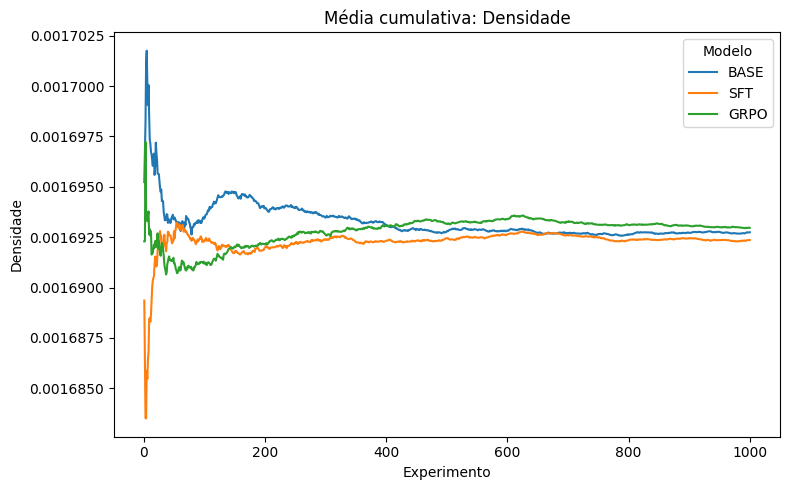
\includegraphics[width=0.75\textwidth]{figure/complete/cumulative-mean/densidade.png}
    \caption{Média cumulativa da Densidade ($\rho$).}
    \label{fig:complete-cumulative-mean-densidade}
\end{figure}

Conforme ilustrado na Figura~\ref{fig:complete-kde-densidade}, as distribuições estimadas por KDE também revelam um comportamento bastante semelhante àquela análisado para o grau médio anteriormente. Do ponto de vista de redes complexas, embora sutis, essa distribuição sugere que os ajustes realizados no modelo base tende a produzir grafos de ativações com maior compactação estrutural, refletida em densidades ligeiramente maiores.

\begin{figure}[h!]
    \centering
    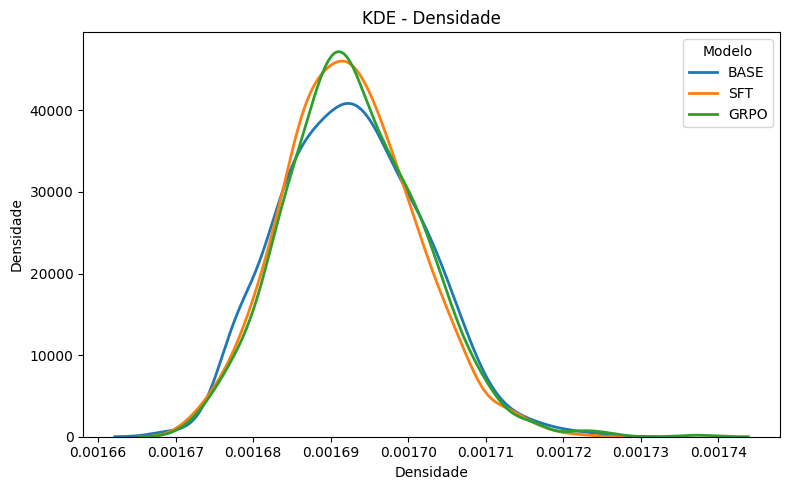
\includegraphics[width=0.75\textwidth]{figure/complete/kde/densidade.png}
    \caption{KDE da Densidade ($\rho$).}
    \label{fig:complete-kde-densidade}
\end{figure}

\subsubsection{Assortatividade ($r$)}

Observa-se que a evolução da média cumulativa da assortatividade, apresentada na Figura~\ref{fig:complete-cumulative-mean-assortatividade}, indica que os três modelos convergem para valores negativos próximos, indicando tendência geral a uma conectividade disassortativa ao longo dos experimentos, com o modelo Base tendendo a apresentar valores médios ligeiramente menos negativos que os modelos ajustados com SFT e GRPO.

\begin{figure}[h!]
    \centering
    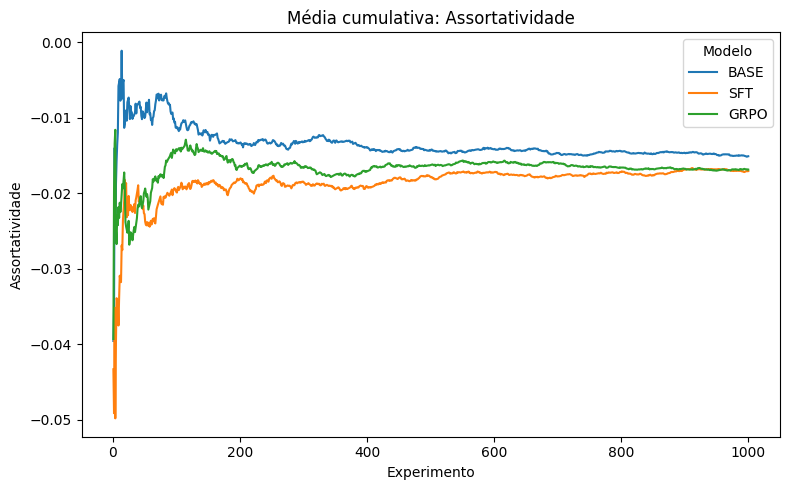
\includegraphics[width=0.75\textwidth]{figure/complete/cumulative-mean/assortatividade.png}
    \caption{Média cumulativa da Assortatividade ($r$).}
    \label{fig:complete-cumulative-mean-assortatividade}
\end{figure}

As distribuições estimadas, na Figura~\ref{fig:complete-kde-assortatividade}, revelam picos concentrados nas regiões próximas de zero e em valores levemente negativos, apesar da proximidade entre as curvas, nota-se que os modelos ajustados com SFT e GRPO exibem distribuições ligeiramente deslocadas e concentradas para regiões mais negativas. Podemos inferir que os ajustes realizados via SFT e GRPO tendem a intensificar, ainda que de forma sutil, a característica disassortativa das redes em comparação ao modelo Base.

\begin{figure}[h!]
    \centering
    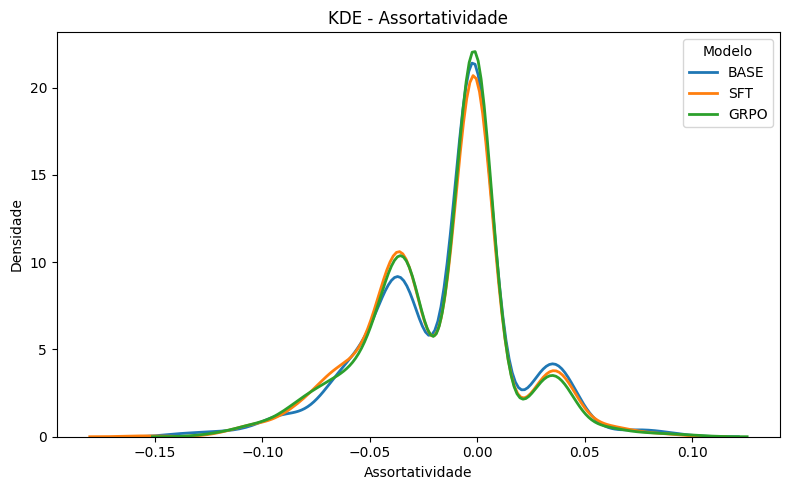
\includegraphics[width=0.75\textwidth]{figure/complete/kde/assortatividade.png}
    \caption{KDE da Assortatividade ($r$).}
    \label{fig:complete-kde-assortatividade}
\end{figure}

\subsubsection{Diâmetro ($D$)}

A Figura~\ref{fig:complete-cumulative-mean-diametro} apresenta a média cumulativa do diâmetro. Os três modelos convergem para valores próximos, com o modelo Base ligeiramente maior e médias ligeiramente menores após SFT e GRPO, sugerindo grafos de ativação um pouco mais compactos que o modelo Base.

\begin{figure}[h!]
    \centering
    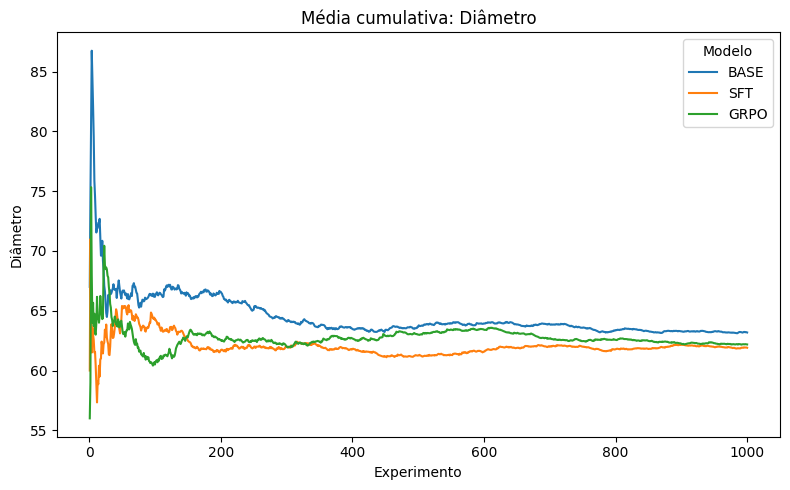
\includegraphics[width=0.75\textwidth]{figure/complete/cumulative-mean/diametro.png}
    \caption{Média cumulativa do Diâmetro ($D$).}
    \label{fig:complete-cumulative-mean-diametro}
\end{figure}

Na Figura~\ref{fig:complete-kde-diametro}, as curvas KDE dos três modelos quase se sobrepõem, nos picos e na leve cauda à direita. Embora as distribuições de densidade sejam visualmente quase idênticas, a análise das médias cumulativas clarifica que os ajustes realizados via SFT e GRPO tendem a reduzir sutilmente o diâmetro médio dos grafos de ativação.

\begin{figure}[h!]
    \centering
    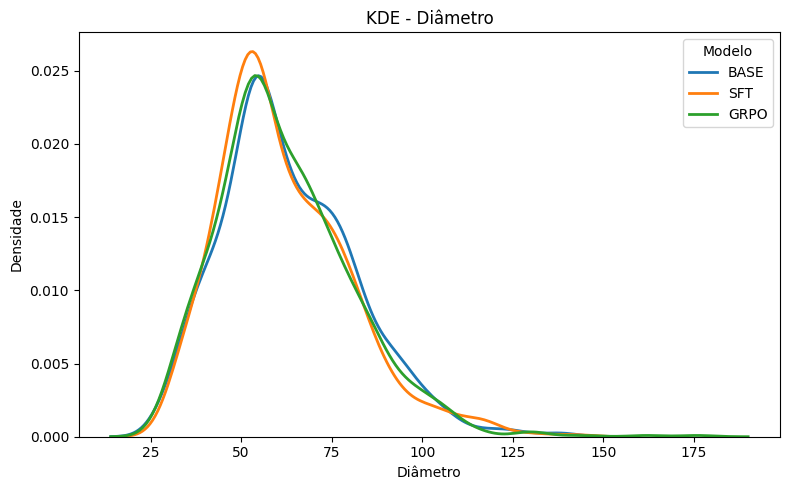
\includegraphics[width=0.75\textwidth]{figure/complete/kde/diametro.png}
    \caption{KDE do Diâmetro ($D$).}
    \label{fig:complete-kde-diametro}
\end{figure}

\subsubsection{Comprimento Médio do Caminho ($\bar{L}$)}

A evolução da média cumulativa do comprimento médio do caminho é apresentada na Figura~\ref{fig:complete-cumulative-mean-path-length}. Pode-se perceber que o modelo Base tende a estabilizar em um valor médio superior em comparação aos modelos ajustados. Em contraste, os modelos SFT e GRPO convergem para valores inferiores e bastante próximos entre si, com o GRPO sendo ligeiramente maior.

\begin{figure}[h!]
    \centering
    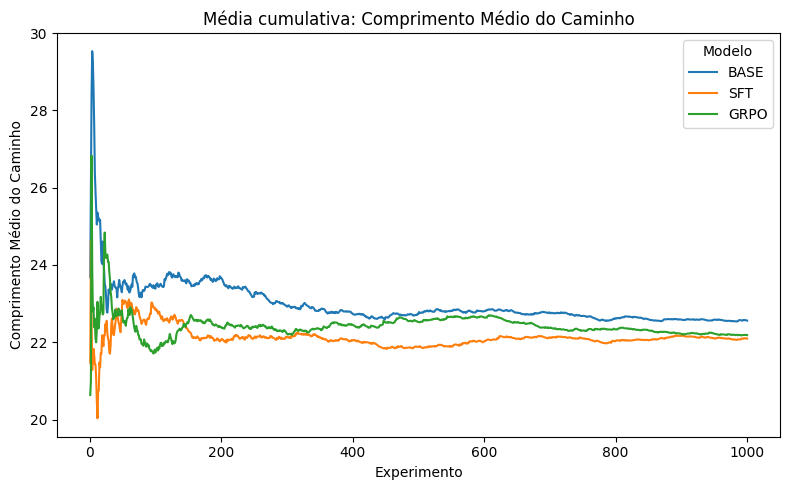
\includegraphics[width=0.75\textwidth]{figure/complete/cumulative-mean/comprimento-medio-caminho.png}
    \caption{Média cumulativa do Comprimento Médio do Caminho ($\bar{L}$).}
    \label{fig:complete-cumulative-mean-path-length}
\end{figure}

As distribuições estimadas por KDE, ilustradas na Figura~\ref{fig:complete-kde-path-length}, condizem com o comportamento observado nas médias cumulativas. As diferenças, picos ligeiramente mais acentuados e o leve deslocamento à esquerda, indicam que os ajustes realizados tendem a reduzir o comprimento médio do caminho na rede de ativações, sugerindo uma maior eficiência na conectividade global quando comparada ao modelo original.

\begin{figure}[h!]
    \centering
    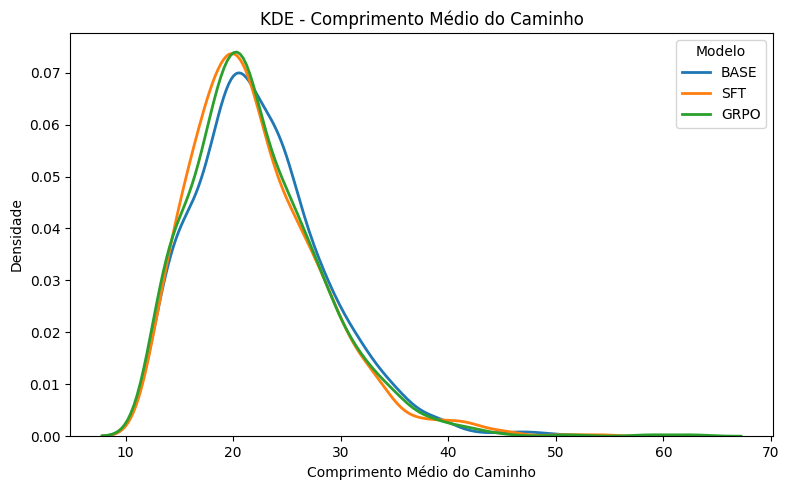
\includegraphics[width=0.75\textwidth]{figure/complete/kde/comprimento-medio-caminho.png}
    \caption{KDE do Comprimento Médio do Caminho ($\bar{L}$).}
    \label{fig:complete-kde-path-length}
\end{figure}

\subsection{Resultados Considerando Apenas as Últimas Cinco Camadas de Ativações}\label{sec:resultados-last-five}

Nesta seção, estão apresentados os resultados obtidos a partir dos experimentos realizados, considerando apenas as últimas cinco camadas do embbeddings gerados aos prompts de labirintos pelos modelos, capturados com a biblioteca LLM-MRI.

\begin{itemize}
    \item \textbf{Número de Nós ($|V|$) e Número de Arestas ($|E|$)}: de modo similar ao observado na seção anterior, não foram observadas diferenças significativas entre os modelos, resultando em distribuições bastante similares e com pouca variabilidade entre os experimentos realizados. Dessa forma, não foram incluídas figuras para estas métricas.
    \item \textbf{Grau Médio ($\bar{k}$), Diâmetro ($D$) e Comprimento Médio do Caminho ($\bar{L}$)}: para estas métricas, não foram observadas diferenças representativas. Foram obtidas distribuições bastante similares entre os modelos, com diferenças mínimas de sobreposição entre as curvas de KDE e valores recorrentes, obtidos durante os experimentos, para as métricas calculadas e médias relativamente reduzidas, se comparadas àquelas obtidas quando consideradas todas as camadas. Sendo assim, figuras para estas métricas não foram incluídas.
\end{itemize}

\subsubsection{Densidade ($\rho$)}

Para a densidade, levando em consideração apenas as últimas cinco camadas de ativações, pode-se observar, na Figura~\ref{fig:last-five-cumulative-mean-densidade}, a evolução da média cumulativa. Apesar de médias estabilizadas próximas entre os modelos, é interessante notar a diferença obtida no valor da média, relativamente maior, quando comparada àquela obtida, para a mesma métrica, considerando o cenário de todas as camadas.

\newpage
\begin{figure}[h!]
    \centering
    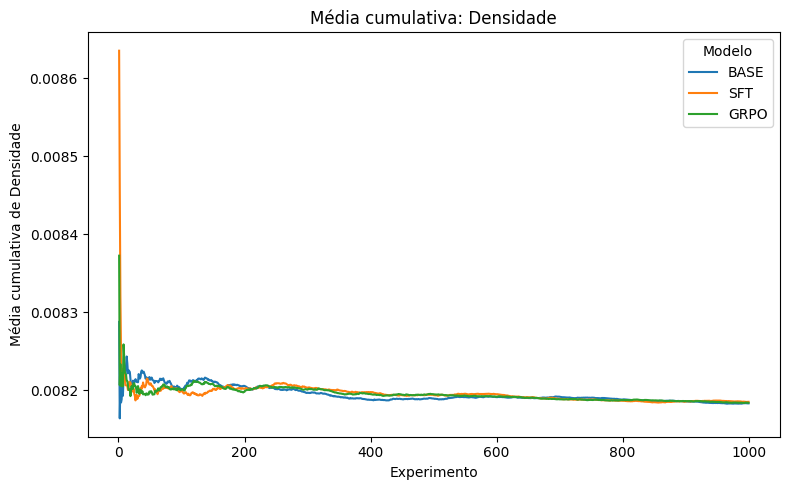
\includegraphics[width=0.75\textwidth]{figure/last-five/cumulative-mean/densidade.png}
    \caption{Média cumulativa da Densidade ($\rho$)}
    \label{fig:last-five-cumulative-mean-densidade}
\end{figure}

Conforme ilustrado na Figura~\ref{fig:last-five-kde-densidade}, as distribuições estimadas por KDE revelam comportamentos muito parecidos entre os modelos. É possível visualizar alguns picos de densidade variados no domínio, evidenciando a repetição de certos valores de densidade ao longo dos experimentos realizados. Apesar disso, as curvas apresentam uma sobreposição considerável, com poucas diferenças visuais entre os modelos e o modelo GRPO apresentando uma leve tendência a valores de densidade mais concentrados.

\begin{figure}[h!]
    \centering
    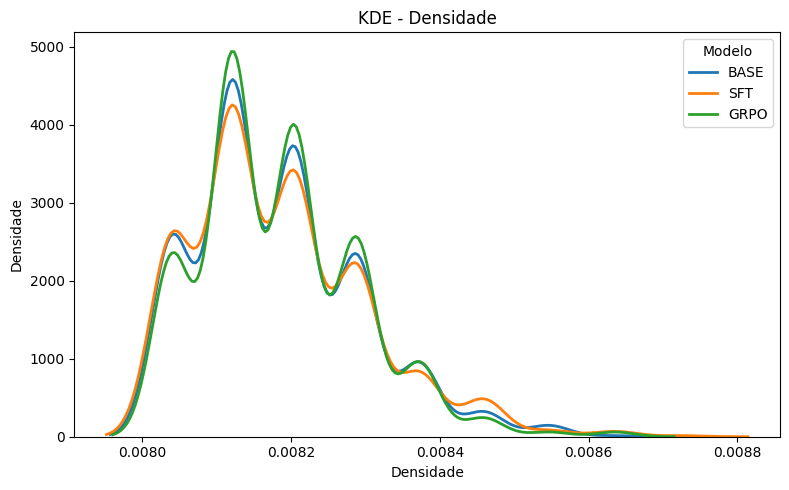
\includegraphics[width=0.75\textwidth]{figure/last-five/kde/densidade.png}
    \caption{KDE da Densidade ($\rho$)}
    \label{fig:last-five-kde-densidade}
\end{figure}

\subsubsection{Assortatividade ($r$)}

É apresentada a evolução da média cumulativa da assortatividade, considerando apenas as últimas cinco camadas, na Figura~\ref{fig:last-five-cumulative-mean-assortatividade}. Percebe-se que o comportamento reflete a tendência observada na análise global em que todos os modelos convergem para valores negativos, caracterizando redes disassortativas. Entretanto, com base no valor estável da média, os modelos Base e ajustados com apresentam uma intensificação da disassortatividade nas camadas finais, quando comparados ao cenário que considera todas as camadas.

\begin{figure}[h!]
    \centering
    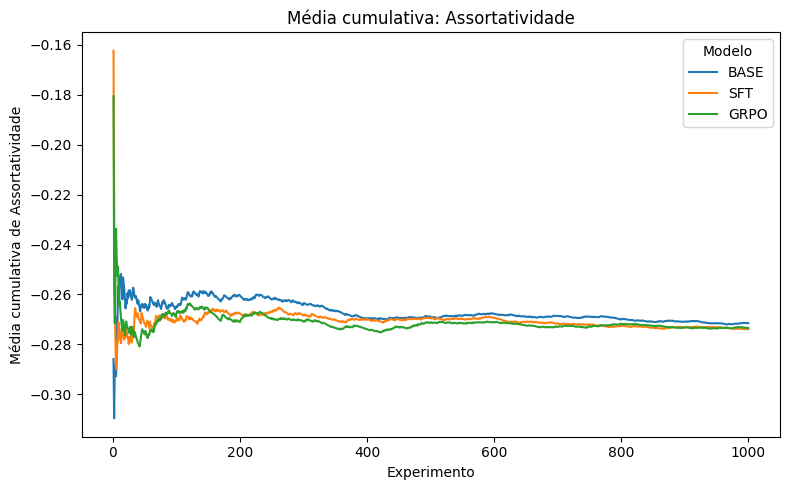
\includegraphics[width=0.8\textwidth]{figure/last-five/cumulative-mean/assortatividade.png}
    \caption{Média cumulativa da Assortatividade ($r$).}
    \label{fig:last-five-cumulative-mean-assortatividade}
\end{figure}

Para a assortatividade, pode-se observar, na Figura~\ref{fig:last-five-kde-assortatividade}, as distribuições estimadas por KDE. De modo distinto, ao que foi apresentado para a assortatividade considerando todas as camadas, as curvas exibem dois picos principais de concentração em regiões mais negativas do domínio, sugerindo uma maior desassortatividade nas redes formadas pelas últimas cinco camadas. Além disso, visualmente, as curvas apresentam uma sobreposição considerável, com poucas diferenças visuais entre os modelos.

\begin{figure}[h!]
    \centering
    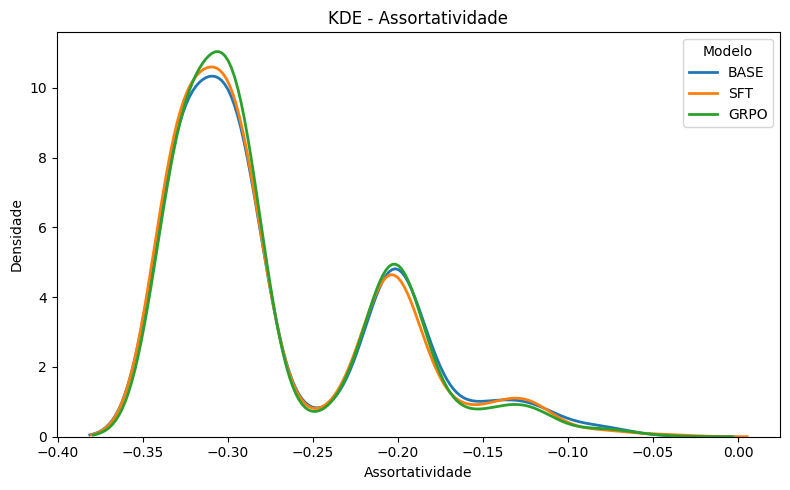
\includegraphics[width=0.66\textwidth]{figure/last-five/kde/assortatividade.png}
    \caption{KDE da Assortatividade ($r$).}
    \label{fig:last-five-kde-assortatividade}
\end{figure}

\subsection{Testes de Significância Estatística}

Para avaliar a significância estatística das diferenças nos gráficos de distribuições e médias observadas para as métricas analisadas, foram realizados testes de hipótese apropriados. Utilizou-se o teste ANOVA para comparar as médias das métricas entre os três modelos, além de Testes t pareados para comparações específicas entre pares de modelos (BASE vs SFT e BASE vs GRPO).

De acordo com os testes, as diferenças, devido ao ajuste dos modelos (SFT ou GRPO), nas estruturas do grafo de ativações neurais dos modelos \textbf{não são estatisticamente significativas} ($p < 0.05$). Do ponto de vista estatístico, isto sugere que as sutis variações observadas, nas distribuições e médias das métricas, podem não ser relevantes o suficiente para serem consideradas significativas.

A Tabela \ref{tab:anova-ttest-full}, a seguir, apresenta os valores \textit{p-value}'s obtidos nos Testes t e ANOVA realizados para as métricas relevantes, considerando todas as camadas dos modelos.

\begin{table}[ht]
\centering
\caption{p-values ANOVA e Testes t pareados (Base vs SFT, Base vs GRPO) – Todas as camadas.}
\label{tab:anova-ttest-full}
\begin{tabular}{|l|c|c|c|}
\hline
Métrica & ANOVA & Base vs SFT & Base vs GRPO \\
\hline
Número de Nós & 0.3125 & 0.3553 & 0.5641 \\
Grau Médio & 0.2682 & 0.2932 & 0.5934 \\
Densidade & 0.2882 & 0.3193 & 0.5821 \\
Assortatividade & 0.3473 & 0.1904 & 0.2345 \\
Diâmetro & 0.2640 & 0.1191 & 0.2272 \\
Comprimento Médio do Caminho & 0.1927 & 0.0851 & 0.1693 \\
\hline
\end{tabular}
\end{table}

Os mesmos testes foram realizados para o cenário considerando apenas as últimas cinco camadas do grafo de ativações neuronais dos modelos, resultados de \textit{p-value}'s descritos na Tabela \ref{tab:anova-ttest-lastfive} e, de forma semelhante, não indicaram diferenças estatisticamente significativas entre o modelo base e os modelos ajustados.

\begin{table}[ht]
\centering
\caption{p-values ANOVA e Testes t pareados (Base vs SFT, Base vs GRPO) – Últimas 5 camadas.}
\label{tab:anova-ttest-lastfive}
\begin{tabular}{|l|c|c|c|}
\hline
Métrica & ANOVA & Bas3 vs SFT & Base vs GRPO \\
\hline
Número de Nós & 0.9282 & 0.7060 & 0.8496 \\
Grau Médio & 0.9257 & 0.7094 & 0.9104 \\
Densidade & 0.9205 & 0.6960 & 0.8902 \\
Assortatividade & 0.6877 & 0.4310 & 0.4893 \\
Diâmetro & 0.4160 & 0.4847 & 0.1785 \\
Comprimento Médio do Caminho & 0.5064 & 0.4727 & 0.2395 \\
\hline
\end{tabular}
\end{table}

Para os dois cenários verificados, os testes de significância estatística da métrica Número de Arestas, por apresentarem valores, no decorrer dos experimentos, muito próximos entre para os diferentes modelos, com pouca variabilidade e muito recorrentes, foi omitida a apresentação dos resultados dos testes estatísticos para esta métrica. A próxima seção apresenta a discussão dos resultados obtidos, interpretando os achados integrando com os objetivos do estudo e das hipóteses formuladas inicialmente.
